\documentclass[11pt]{article}
\usepackage[margin=1in]{geometry}
\usepackage[T1]{fontenc}
\usepackage{amsmath,amssymb,graphicx,booktabs,enumitem,xcolor,caption}
\usepackage[round]{natbib}
\usepackage[colorlinks=true,urlcolor=blue,citecolor=blue]{hyperref}
\title{Progress Report\\[4pt]\large Single-Image / Single-Video Overfit Neural Compression\\Implicit Neural Codec -- Project 3}
\author{
Ganna Hatem Deghady\\2500014
\and
Gannah Mohamed Ghamry\\2501779
\and
Nour Ayman AbouElMakarem\\2501913
}
\date{Milestone 2 -- November 15, 2026\\CSE681 -- Digital Image Processing}
\begin{document}
\maketitle
\begin{abstract}
This milestone extends the single-image Fourier-feature network from Milestone 1 into a working image codec evaluated on all 24 original-resolution Kodak images. The implementation quantizes network parameters, writes packed weight files, and reconstructs images from those files without the source image or training checkpoint. Experiments cover three network widths and three weight precisions, together with reproduced JPEG and HEVC-intra baselines. At 8-bit precision, the neural models achieve mean RGB PSNR values of 22.73, 24.13, and 25.63 dB at 0.084, 0.234, and 0.784 bpp, respectively. HEVC-intra provides stronger preliminary rate-distortion performance; the main outcome is a reproducible measurement of the capacity, quantization, and CPU encoding-cost trade-offs of the simple implicit codec.
\end{abstract}
\section{Recap}
We investigate compression by fitting a small coordinate network separately to each image and storing its parameters. The approach is inspired by COIN \citep{coin}, but uses a Fourier-feature ReLU MLP rather than the original sine-activation architecture. C3 \citep{c3} provides broader context for overfitted compression; the current implementation does not reproduce its hierarchical latents or learned entropy model. M1 demonstrated reconstruction on a resized image. M2 targets a real stored representation, all 24 Kodak images at their native dimensions, and a parameter-count sweep compared with JPEG and HEVC-intra. Video remains planned for M3.
\paragraph{Code and reproducibility.}
The source code, experimental results, and instructions
for reproducing the experiments are available at:
\url{https://github.com/GannaHatem/neural-image-compression-cse681}.
\section{Implementation Status}
\subsection{Baseline Reproduction}
We evaluate on the Kodak image suite \citep{kodak},
using JPEG \citep{jpeg} and HEVC-intra \citep{hevc}
as classical baselines.
Both classical baselines use the same 8-bit RGB reference images as the neural experiments, without resizing or cropping. JPEG uses Pillow at qualities 1, 3, 5, 10, 20, 30, 50, 70, and 90 with chroma subsampling disabled. HEVC uses FFmpeg/libx265, the medium preset, yuv444p, and one intra-coded frame at CRF 10, 20, 30, 40, 45, and 51. The x265 settings specify keyint=1, min-keyint=1, scenecut=0, pools=4, and frame-threads=1. The FFmpeg version output is included in the package. HEVC is converted back to RGB before quality measurement; its RGB/YUV conversion is part of the baseline pipeline.

JPEG rate counts the complete JPEG file. HEVC rate counts the raw HEVC stream, including parameter-set headers. Results comprise 216 JPEG records and 144 HEVC records.
\subsection{Our Method}
For an image of dimensions $H\times W$, the network maps normalized coordinates $(x,y)\in[0,1]^2$ to RGB. For each coordinate component, the input features are $\sin(2^k\pi x)$ and $\cos(2^k\pi x)$, with $k=0,\ldots,7$, yielding 32 features. Three hidden ReLU layers of width $w$ precede a three-channel sigmoid output. Widths 32, 64, and 128 contain 3,267, 10,627, and 37,635 trainable parameters.

Each image/width combination is fitted for 5,000 Adam steps at learning rate $10^{-3}$ using batches of 2,048 randomly sampled pixel coordinates, with replacement. The seed is reset to 42 for each fit, and PyTorch uses four CPU threads. Training minimizes RGB MSE. The hardware is an AMD Ryzen 5 7520U laptop with 8 GB installed RAM; the recorded environment is Python 3.10.0, PyTorch 2.14.1+cpu, and NumPy 2.2.6. There are 72 independent fits. Each fit is reused to evaluate 6-, 8-, and 10-bit weights, producing 216 neural records.

For each parameter tensor, uniform min--max quantization produces integer symbols:
\begin{equation}
q=\operatorname{round}\left(\frac{\theta-\theta_{\min}}{\theta_{\max}-\theta_{\min}}(2^b-1)\right),\qquad
\hat\theta=\theta_{\min}+\frac{q}{2^b-1}(\theta_{\max}-\theta_{\min}).
\end{equation}
Constant tensors are represented by zero symbols and the shared endpoint. Symbols are packed into $b$ bits each, with byte padding per tensor. A magic identifier, header length, and JSON metadata describe the architecture, image dimensions, tensor shapes, and endpoints. No entropy coding is applied. The decoder creates a fresh network from this metadata and reconstructed weights; it does not load a training checkpoint. Reconstruction is evaluated in chunks of 4,096 pixels and rounded/clipped to 8-bit RGB.
\section{Preliminary Results}
\subsection{Protocol and Validation}
All images have 393,216 pixels (768$\times$512 or 512$\times$768). Metrics are
\begin{equation}
\mathrm{bpp}=\frac{8\,\mathrm{file\ bytes}}{HW},\qquad
\mathrm{PSNR}=10\log_{10}\frac{255^2}{\mathrm{MSE}_{RGB}}.
\end{equation}
MSE averages over all pixels and RGB channels. Tables and curves report the arithmetic mean of per-image PSNR and bpp. Native reference pixels agree between all three methods. All 576 records were checked against saved reconstructions and file sizes. Neural payload lengths were checked against their metadata. An independent NumPy decoder spot check on kodim01, width 64, 8-bit weights agreed with the PNG within one intensity level; approximately 0.000933\% of channel values differed. This spot check does not independently validate decoding of every stream.

Per-image optimization deliberately uses the evaluated image, so a conventional disjoint training/test split is not applicable. The architecture and budget are fixed across images for this sweep; results are preliminary benchmark measurements, not evidence of generalization to unseen images. Curves join sampled settings, and mean-rate points are not exact per-image matched-rate comparisons.
\begin{table}[ht]
\centering\caption{Neural codec on all 24 images, 5,000 steps per fit. Training time is shared across precisions for each image/width.}
\begin{tabular}{rrrrr}\toprule
Width & Weight bits & Mean bpp & Mean PSNR (dB) & Train/image (s)\\\midrule
32 & 6 & 0.0675 & 22.20 & 19.07\\
32 & 8 & 0.0842 & 22.73 & 19.07\\
32 & 10 & 0.1009 & 22.77 & 19.07\\
64 & 6 & 0.1799 & 23.47 & 28.24\\
64 & 8 & 0.2340 & 24.13 & 28.24\\
64 & 10 & 0.2881 & 24.16 & 28.24\\
128 & 6 & 0.5923 & 24.98 & 52.89\\
128 & 8 & 0.7838 & 25.63 & 52.89\\
128 & 10 & 0.9753 & 25.69 & 52.89\\\bottomrule
\end{tabular}
\end{table}
\begin{table}[ht]
\centering\caption{Selected reproduced classical baseline points, averaged over the same 24 images. Settings are not rate-matched to the neural codec.}
\begin{tabular}{llrr}\toprule
Method & Setting & Mean bpp & Mean PSNR (dB)\\\midrule
JPEG & Q=1 & 0.2667 & 21.55\\
JPEG & Q=10 & 0.4246 & 26.94\\
JPEG & Q=30 & 0.7843 & 30.91\\
HEVC-intra & CRF=51 & 0.0875 & 24.41\\
HEVC-intra & CRF=45 & 0.1610 & 26.93\\
HEVC-intra & CRF=40 & 0.2994 & 29.55\\
HEVC-intra & CRF=30 & 0.9267 & 35.51\\\bottomrule
\end{tabular}
\end{table}
\begin{figure}[ht]\centering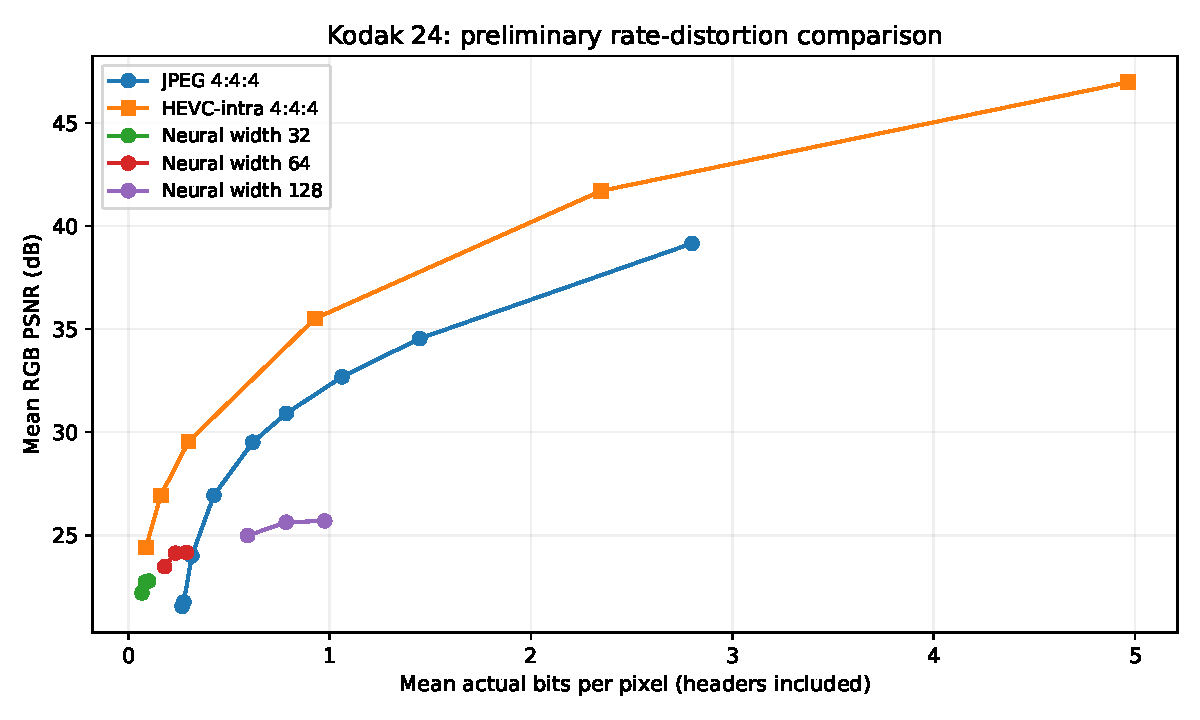
\includegraphics[width=\linewidth]{rd_all.pdf}
\caption{Measured RD curves. Each point averages all 24 Kodak images. Neural curves vary weight precision within one width. Lines connect sampled operating points and do not imply exact matched-rate measurements.}\end{figure}
\subsection{Interpolated Matched-Rate Comparison}

For each image and neural configuration, baseline RGB
PSNR was linearly interpolated between measured baseline
points at the neural codec's actual bitrate.
No extrapolation was used. Configurations outside the
measured baseline range were excluded, and the number
of supported images is reported for each comparison.
Positive PSNR differences favor the neural codec;
negative differences favor the baseline.

\begin{table}[htbp]
\centering
\small
\caption{Interpolated per-image matched-bpp comparison. $\Delta$PSNR is neural minus baseline; positive values favor the neural codec. Means use only supported images. No extrapolation is used.}
\label{tab:matched_bpp}
\begin{tabular}{rrrrrr}
\toprule
Width & Bits & JPEG images & JPEG $\Delta$dB & HEVC images & HEVC $\Delta$dB \\
\midrule
32 & 6 & 0/24 & -- & 1/24 & -0.13 \\
32 & 8 & 0/24 & -- & 12/24 & -1.74 \\
32 & 10 & 0/24 & -- & 21/24 & -2.46 \\
64 & 6 & 0/24 & -- & 24/24 & -4.18 \\
64 & 8 & 0/24 & -- & 24/24 & -4.56 \\
64 & 10 & 21/24 & +1.06 & 24/24 & -5.32 \\
128 & 6 & 24/24 & -4.51 & 24/24 & -7.93 \\
128 & 8 & 24/24 & -5.50 & 24/24 & -8.68 \\
128 & 10 & 24/24 & -6.67 & 24/24 & -9.80 \\
\bottomrule
\end{tabular}
\end{table}
At width 64 with 10-bit weights, the neural codec
exceeds interpolated JPEG PSNR by 1.06 dB on the
21 supported images. However, HEVC-intra performs
better on every evaluated neural configuration
within the supported rate range. Coverage differs
between configurations, so these averages must
not be interpreted as comparisons over identical
image subsets.
\subsection{Findings}
Increasing width improves reconstruction quality, but increases rate and fitting time. At 8 bits, moving from width 32 to 128 raises mean PSNR by 2.89 dB while raising mean bitrate from 0.0842 to 0.7838 bpp. The measured training total across the 72 fits is 40.08 minutes. Training must not be counted three times for the three weight precisions. Mean neural decoding times range from approximately 0.17 to 0.61 s across the settings.

Increasing precision from 8 to 10 bits improves mean PSNR by only 0.038, 0.033, and 0.065 dB at widths 32, 64, and 128, respectively. Six-bit weights lose approximately 0.54--0.66 dB relative to 8-bit weights. These measurements support 8 bits as a practical compromise for this implementation and optimization budget.

The widest 8-bit model reaches 25.63 dB at 0.7838 bpp, whereas JPEG Q=30 reaches 30.91 dB at 0.7843 bpp. These nearly equal mean rates show a substantial quality gap, although the rates differ on individual images. HEVC CRF=51 reaches 24.41 dB at 0.0875 bpp, compared with 22.73 dB at 0.0842 bpp for the smallest 8-bit model. Smaller neural models operate below the minimum measured JPEG rates on many images; claims of exact matched-rate superiority are therefore inappropriate there. The current simple codec does not establish superiority over the classical baselines.

Timing protocols also differ: JPEG encoding is measured in memory, HEVC encoding includes FFmpeg process and file overhead, and neural encoding includes fitting plus weight serialization. These are practical pipeline timings rather than an isolated implementation-speed comparison.
\begin{figure}[p]\centering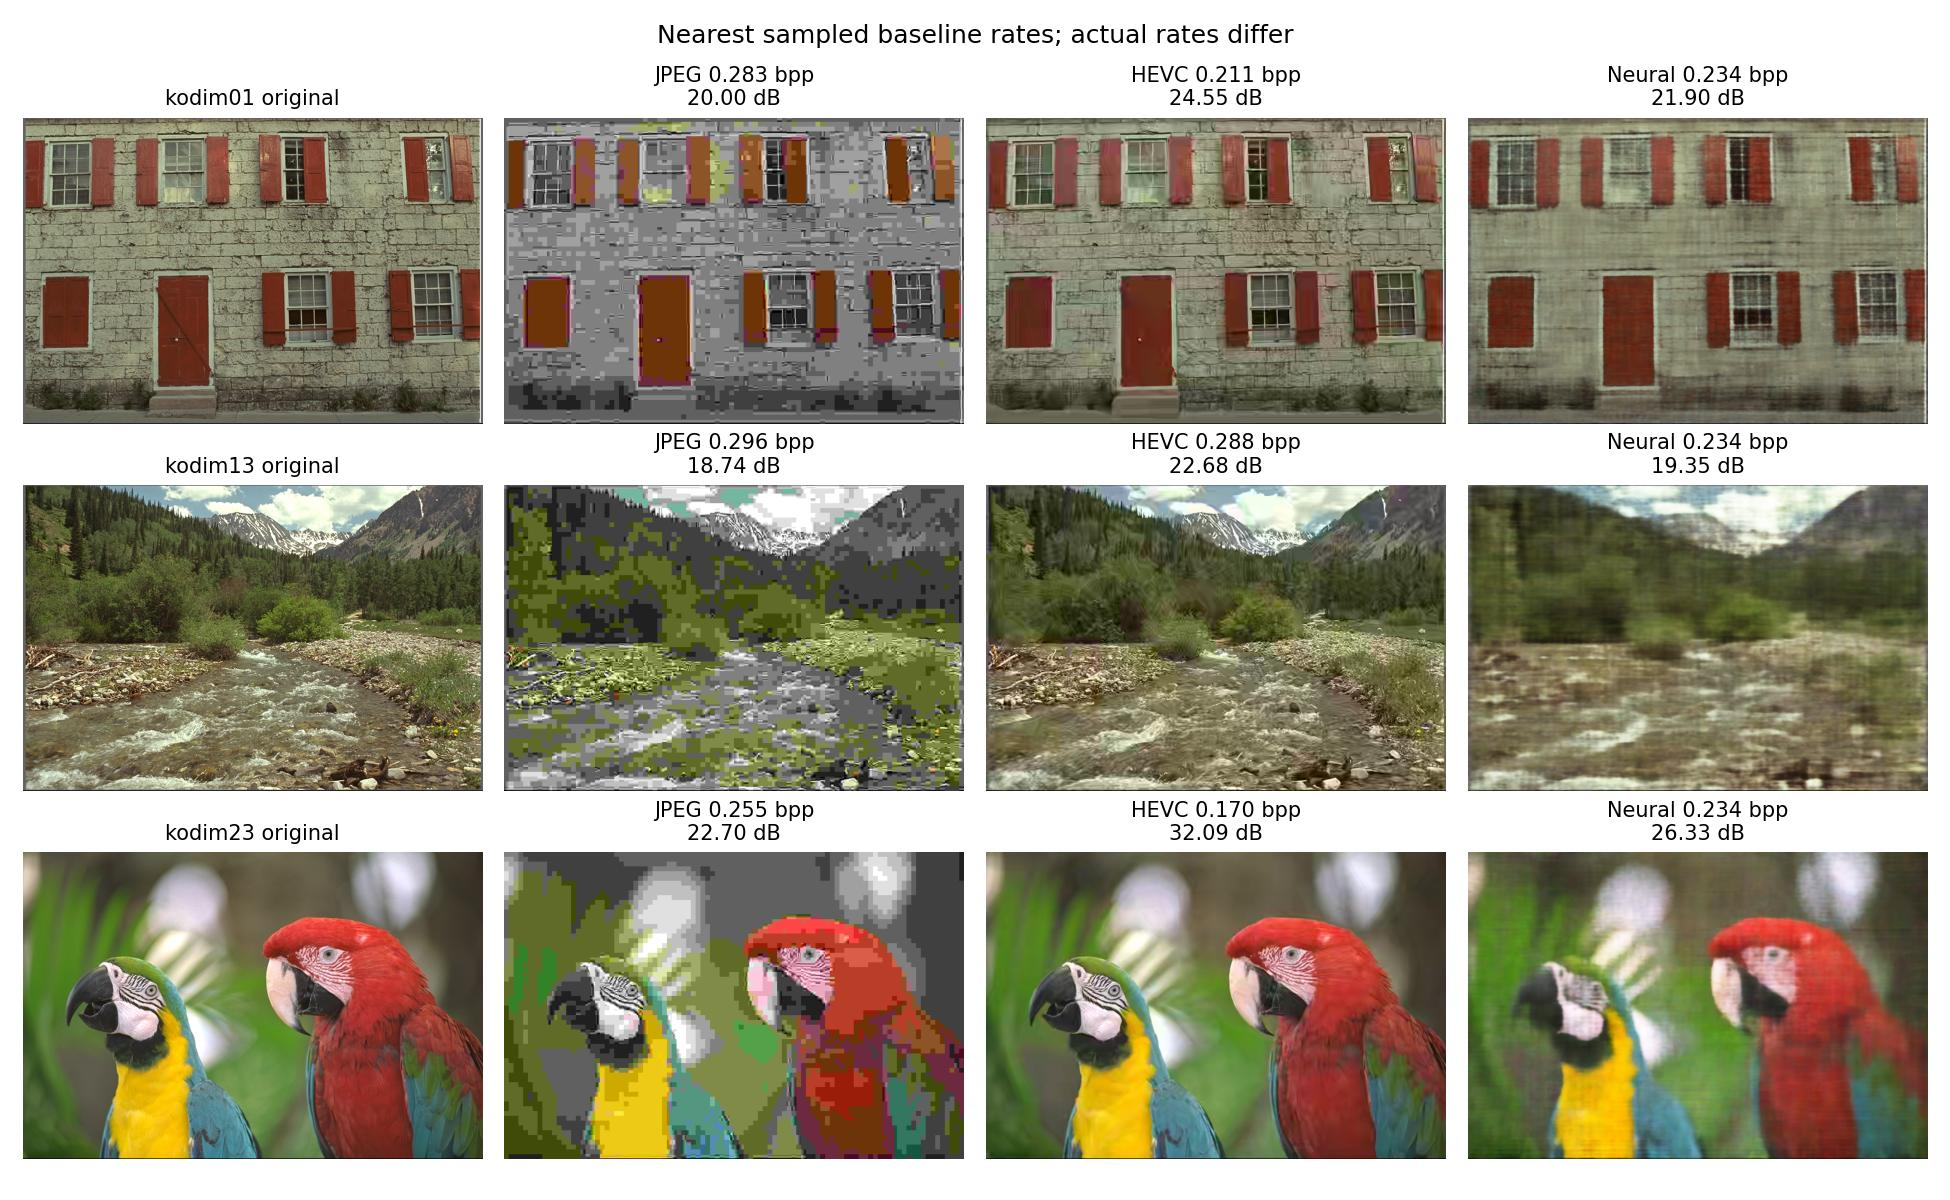
\includegraphics[width=\linewidth]{examples_all.jpg}
\caption{Three illustrative images (kodim01, kodim13, kodim23), comparing originals, JPEG, HEVC-intra, and the width-64/8-bit codec. Baselines use the nearest sampled rate to the neural rate for each image; actual bpp and PSNR are shown. Rates differ, so this grid is qualitative context rather than a strict equal-rate test.}\end{figure}
\section{Challenges \& Deviations from the M1 Plan}
The full-resolution sweep and real encode/decode path are complete. The batch size was reduced from 4,096 to 2,048 to suit the CPU laptop. The weight format uses descriptive JSON metadata rather than the compact fixed-header estimate proposed in M1; all actual overhead is counted. Additional low-quality JPEG points and high-CRF HEVC points extend baseline coverage. The former estimated weight bpp is no longer used as a measured rate.

The principal limitation is weak rate-distortion performance at larger widths under the fixed 5,000-step budget. Insufficient fitting time and the restricted coordinate-MLP representation are plausible explanations, but the present experiment does not isolate their individual effects. No claim is made that additional steps alone will close the gap. Entropy coding, video, and a systematic training-budget ablation remain unimplemented.
\clearpage
\section{Updated Work Breakdown \& MVP Status}
The M1 minimum-viable image-codec deliverable has been
reached. The codec quantizes and stores network weights,
decodes the resulting files without the original image,
and evaluates all 24 Kodak images against JPEG and
HEVC-intra. The video extension remains planned for
Milestone 3.

\begin{itemize}
    \begin{table}[htbp]
\centering
\small
\caption{Updated milestone task allocation.}
\label{tab:tasks}
\begin{tabular}{@{}p{0.13\linewidth}
                  p{0.26\linewidth}
                  p{0.26\linewidth}
                  p{0.26\linewidth}@{}}
\toprule
\textbf{Milestone} &
\textbf{Ganna Hatem} &
\textbf{Gannah Ghamry} &
\textbf{Nour Ayman} \\
\midrule

M2 completed &
Co-led implementation and experiments; prepared data,
ran baselines, and checked reconstructed images. &
Co-led implementation and experiments; ran neural-codec
experiments and reviewed quality and bitrate results. &
Reviewed the report, cross-checked tables against CSV
results, and checked references. \\

\addlinespace
M3 planned &
Prepare the UVG video patch and run the classical
video baseline. &
Evaluate video reconstruction quality, bitrate,
and timing; prepare comparison plots. &
Lead the video-codec extension and investigate
parameter entropy coding, with team support. \\

\bottomrule
\end{tabular}
\end{table}
\end{itemize}
Ganna and Gannah shared the main implementation and
experimental workload. The team reviewed the final
Milestone 2 deliverables together.

\section{Next Steps}
First, fix a small development subset and compare longer fitting budgets to measure whether training time improves the neural RD curve. Second, evaluate a lossless compressor on the packed parameter payload and count all resulting overhead. Third, implement the M1 video plan: a coordinate network using $(x,y,t)$ for a 30-frame, 180$\times$240 HoneyBee patch, with a reproduced HEVC video baseline. Finally, document failures, verify standalone decoding, and prepare the M3 demonstration. Any expanded experiment should preserve this M2 run as the original fixed-budget comparison.
\paragraph{AI assistance and team review.} 
AI tools assisted with code scaffolding, debugging,
metric checking, and report drafting. The team executed
the experiments locally. The reported numerical results
were calculated from the resulting files and reconstructed
images.

\bibliographystyle{unsrtnat}
\bibliography{references}

\end{document}
